% Options for packages loaded elsewhere
\PassOptionsToPackage{unicode}{hyperref}
\PassOptionsToPackage{hyphens}{url}
%
\documentclass[
  10pt,
  b5paper,
  oneside]{book}
\usepackage{amsmath,amssymb}
\usepackage{lmodern}
\usepackage{iftex}
\ifPDFTeX
  \usepackage[T1]{fontenc}
  \usepackage[utf8]{inputenc}
  \usepackage{textcomp} % provide euro and other symbols
\else % if luatex or xetex
  \usepackage{unicode-math}
  \defaultfontfeatures{Scale=MatchLowercase}
  \defaultfontfeatures[\rmfamily]{Ligatures=TeX,Scale=1}
\fi
% Use upquote if available, for straight quotes in verbatim environments
\IfFileExists{upquote.sty}{\usepackage{upquote}}{}
\IfFileExists{microtype.sty}{% use microtype if available
  \usepackage[]{microtype}
  \UseMicrotypeSet[protrusion]{basicmath} % disable protrusion for tt fonts
}{}
\makeatletter
\@ifundefined{KOMAClassName}{% if non-KOMA class
  \IfFileExists{parskip.sty}{%
    \usepackage{parskip}
  }{% else
    \setlength{\parindent}{0pt}
    \setlength{\parskip}{6pt plus 2pt minus 1pt}}
}{% if KOMA class
  \KOMAoptions{parskip=half}}
\makeatother
\usepackage{xcolor}
\usepackage{longtable,booktabs,array}
\usepackage{calc} % for calculating minipage widths
% Correct order of tables after \paragraph or \subparagraph
\usepackage{etoolbox}
\makeatletter
\patchcmd\longtable{\par}{\if@noskipsec\mbox{}\fi\par}{}{}
\makeatother
% Allow footnotes in longtable head/foot
\IfFileExists{footnotehyper.sty}{\usepackage{footnotehyper}}{\usepackage{footnote}}
\makesavenoteenv{longtable}
\usepackage{graphicx}
\makeatletter
\def\maxwidth{\ifdim\Gin@nat@width>\linewidth\linewidth\else\Gin@nat@width\fi}
\def\maxheight{\ifdim\Gin@nat@height>\textheight\textheight\else\Gin@nat@height\fi}
\makeatother
% Scale images if necessary, so that they will not overflow the page
% margins by default, and it is still possible to overwrite the defaults
% using explicit options in \includegraphics[width, height, ...]{}
\setkeys{Gin}{width=\maxwidth,height=\maxheight,keepaspectratio}
% Set default figure placement to htbp
\makeatletter
\def\fps@figure{htbp}
\makeatother
\setlength{\emergencystretch}{3em} % prevent overfull lines
\providecommand{\tightlist}{%
  \setlength{\itemsep}{0pt}\setlength{\parskip}{0pt}}
\setcounter{secnumdepth}{5}
\usepackage{booktabs}
\usepackage{amsthm}
\makeatletter
\let\stdl@chapter\l@chapter
\renewcommand*{\l@chapter}[2]{%
  \stdl@chapter{\textcolor{astral}{#1}}{\textcolor{astral}{#2}}}

\def\thm@space@setup{%
  \thm@preskip=5cm
  \thm@postskip=\thm@preskip

}
\usepackage{graphicx}
\usepackage{afterpage}

\newcommand\blankpage{%
    \null
    \thispagestyle{empty}%
    \addtocounter{page}{-1}%
    \newpage}

\usepackage{amssymb}
\usepackage{amsmath}
%\pagestyle{plain} % default for report

\usepackage{etoolbox}
\makeatletter
\patchcmd{\@makechapterhead}{50\p@}{-24pt}{}{}
\patchcmd{\@makeschapterhead}{50\p@}{-24pt}{}{}
\makeatother

\makeatother
\usepackage{sectsty}

\definecolor{astral}{RGB}{153, 61, 15}
\allsectionsfont{\sffamily\color{astral}}


\usepackage{fancyhdr}
\usepackage{pdfpages}

\renewcommand{\headrulewidth}{0.5pt}
\renewcommand{\headrule}{\hbox to\headwidth{\color{astral}\leaders\hrule height \headrulewidth\hfill}}


\setlength{\headheight}{5pt}

\fancyhf{}
\fancyhead[EL]{\nouppercase\leftmark}
\fancyhead[OR]{\nouppercase\rightmark}
\fancyhead[ER,OL]{\thepage}

\usepackage{multicol}
\usepackage{hyperref}
\usepackage{longtable}
\usepackage{array}
\usepackage{multirow}
\usepackage{wrapfig}
\usepackage{float}
\usepackage{colortbl}
\usepackage{pdflscape}
\usepackage{tabu}
\usepackage{threeparttable}
\usepackage{adjustbox}
\usepackage{rotating}
\usepackage{tablefootnote}
\usepackage[normalem]{ulem}
% empty pages betwen chapters
\usepackage{emptypage}


\makeatletter
\makeatother

\renewcommand{\listfigurename}{Figures}
\renewcommand{\listtablename}{Tables}

\usepackage[sectionbib]{chapterbib}

%% List of Abbreviations
\usepackage{nomencl}
\makenomenclature
\renewcommand{\nomname}{Acronyms}
%% to update run makeindex on docs folder and move results to / folder
%% see nomencl manual
%% e.g. makeindex SOCMapping.nlo -s nomencl.ist -o SOCMapping.nls

%% index
\usepackage{imakeidx}
\makeindex

\usepackage{xspace}

% no title page
\AtBeginDocument{\let\maketitle\relax}
\hypersetup{
	colorlinks=true,
	linkcolor=astral,
	filecolor=astral,
	urlcolor=astral,
	citecolor=astral
}
\AtBeginDocument{\renewcommand{\chaptername}{Chapter}}
\usepackage{titling}
\usepackage{natbib}
\usepackage{pdfpages}
\usepackage{fancyhdr}
\usepackage{booktabs}
\usepackage{longtable}
\usepackage{subfig}
\usepackage{array}
\usepackage{amsmath}
\usepackage{multirow}
\usepackage{wrapfig}
\usepackage{bookmark}
\usepackage[utf8]{inputenc}
\usepackage{float}
\usepackage{colortbl}
\usepackage{pdflscape}
\usepackage{tabu}
\usepackage{threeparttable}
\usepackage{threeparttablex}
\usepackage[normalem]{ulem}
\usepackage{makecell}
\usepackage{xcolor}
\DeclareUnicodeCharacter{2212}{\textendash}
\usepackage{rotating, graphicx}
\ifLuaTeX
  \usepackage{selnolig}  % disable illegal ligatures
\fi
\IfFileExists{bookmark.sty}{\usepackage{bookmark}}{\usepackage{hyperref}}
\IfFileExists{xurl.sty}{\usepackage{xurl}}{} % add URL line breaks if available
\urlstyle{same} % disable monospaced font for URLs
\hypersetup{
  pdftitle={ Technical Manual for Global Soil Nutrient and Nutrient Budgets map (GSNmap)},
  pdfauthor={Angelini, M.E, Luotto, I., Rodriguez Lado, L., Mainka, M., Yigini, Y., Tong, Y.},
  hidelinks,
  pdfcreator={LaTeX via pandoc}}

\title{
Technical Manual for Global Soil Nutrient and Nutrient Budgets map (GSNmap)}
\usepackage{etoolbox}
\makeatletter
\providecommand{\subtitle}[1]{% add subtitle to \maketitle
  \apptocmd{\@title}{\par {\large #1 \par}}{}{}
}
\makeatother
\subtitle{version 0.2}
\author{Angelini, M.E, Luotto, I., Rodriguez Lado, L., Mainka, M., Yigini, Y., Tong, Y.}
\date{26-Oct-2022}

\begin{document}
\maketitle

\pagestyle{plain}
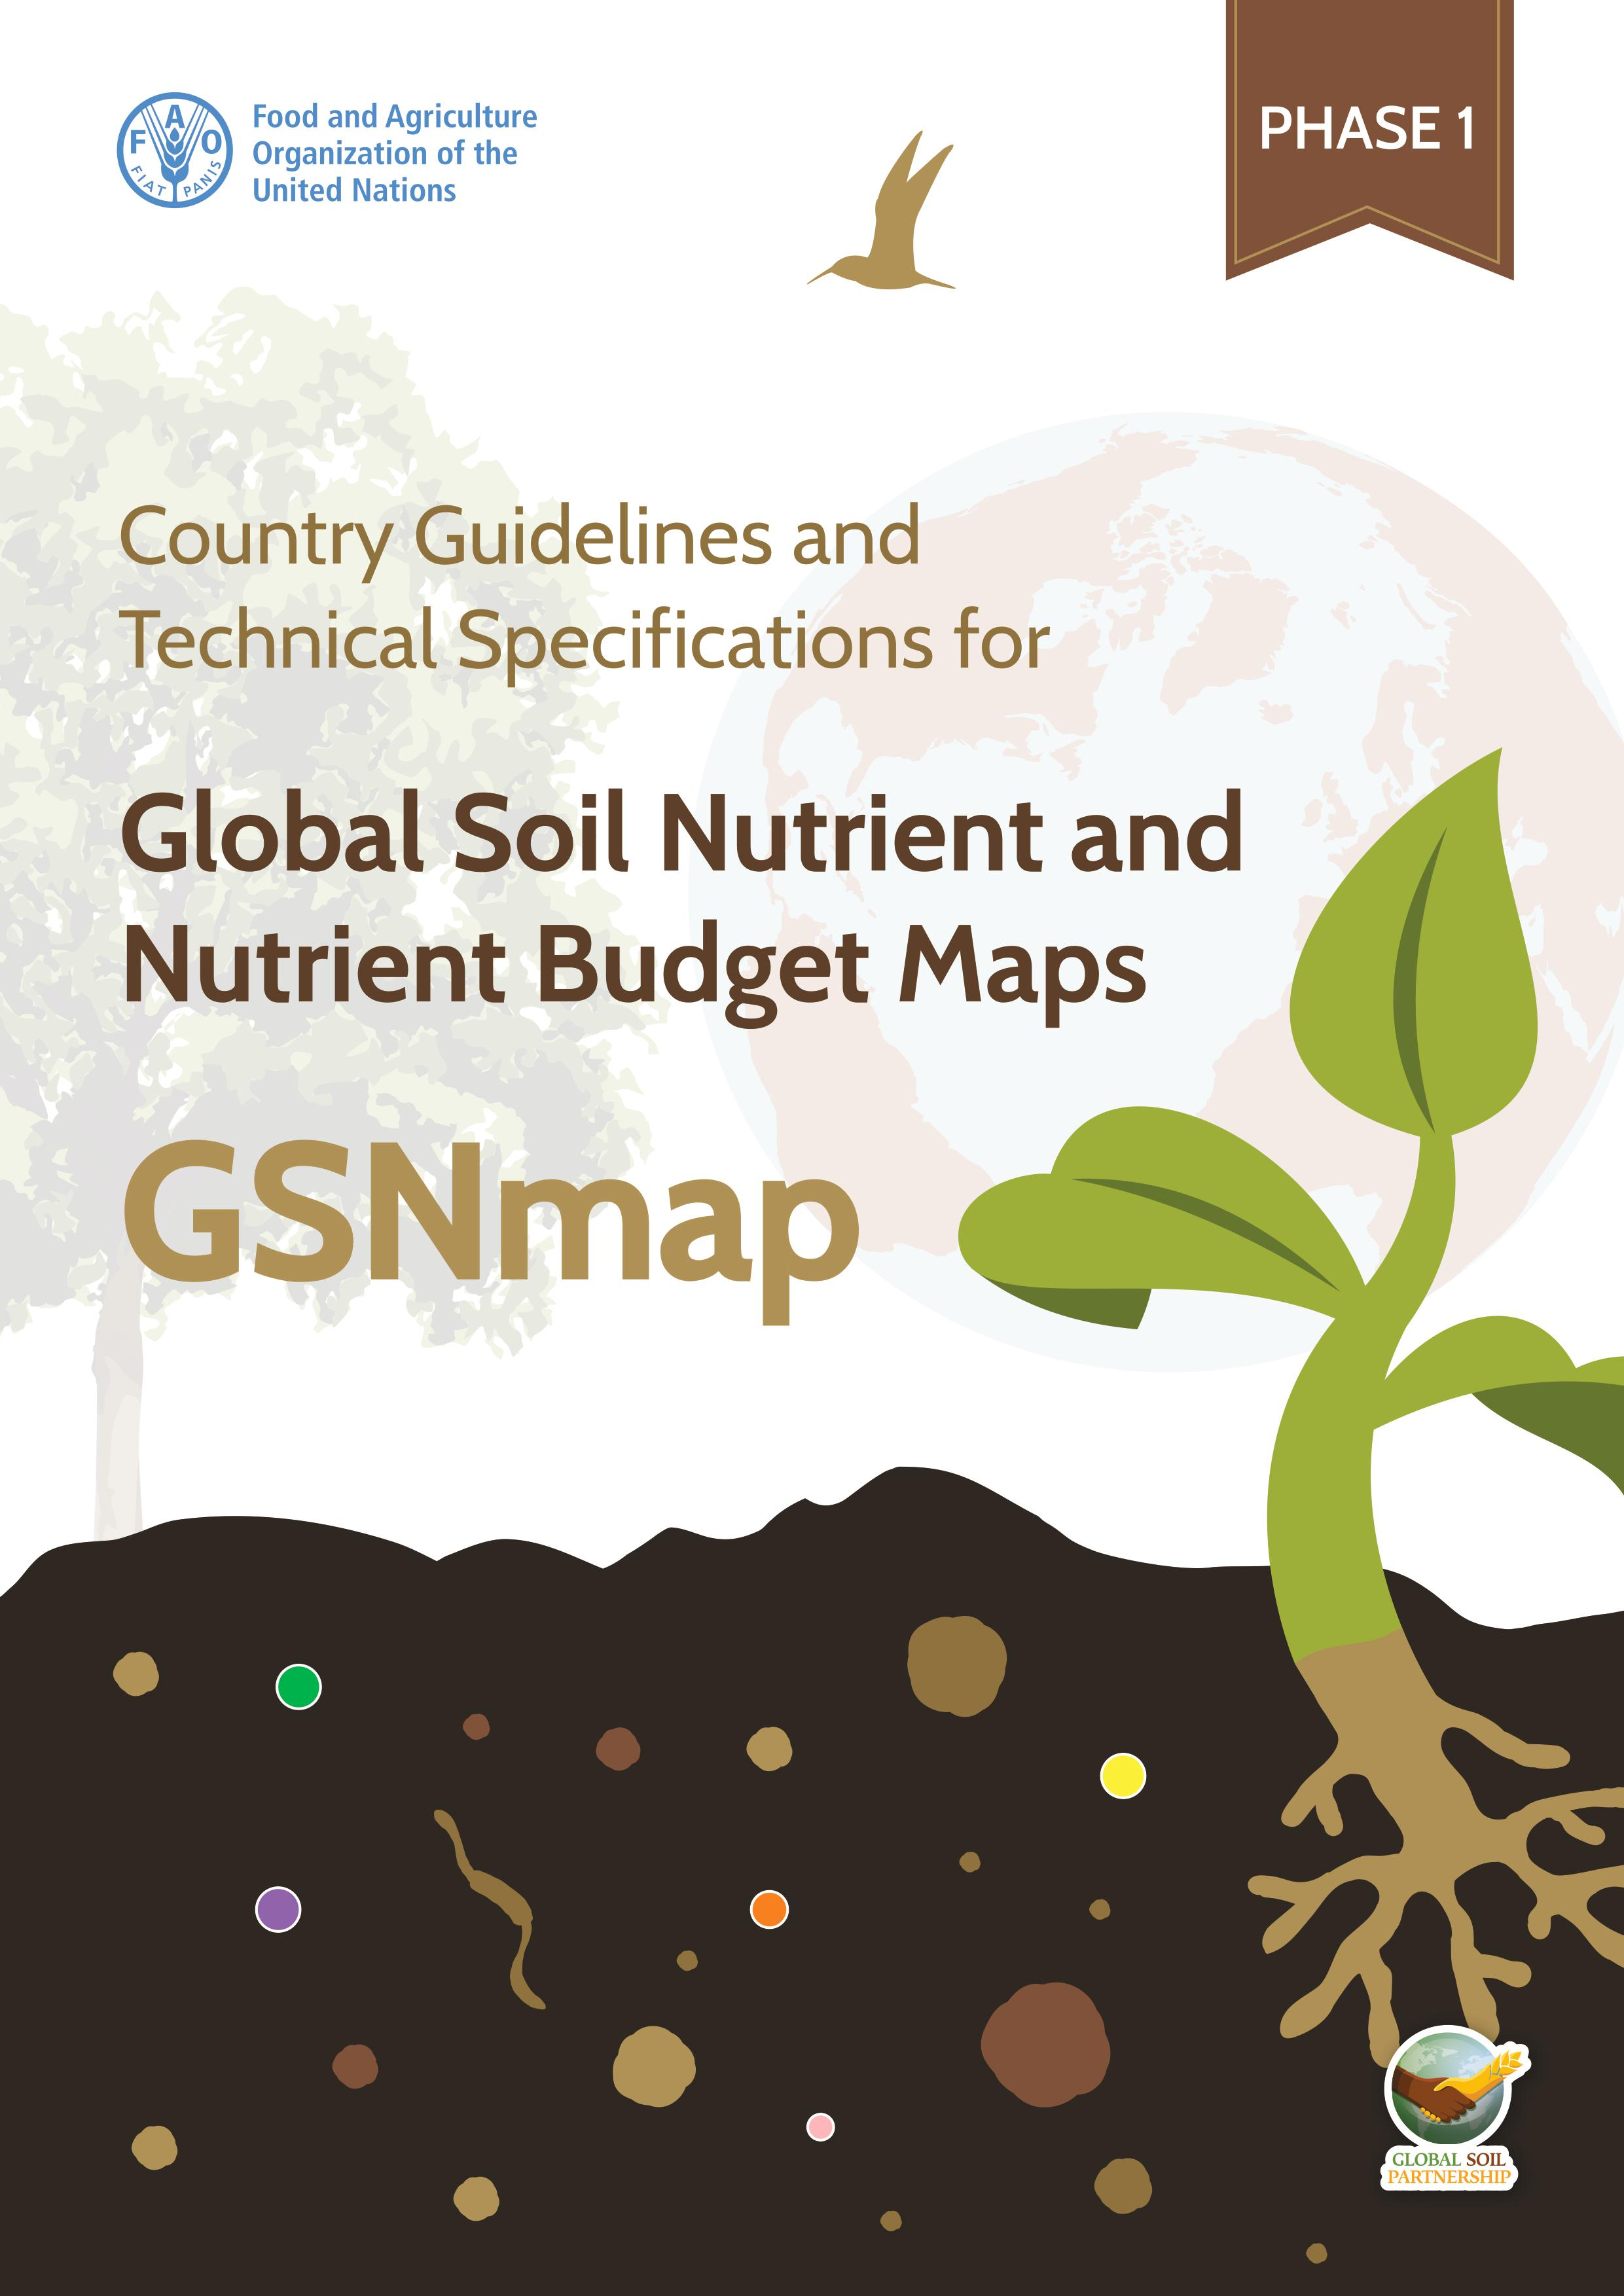
\includepdf{images/frontcover.pdf}
\afterpage{\blankpage}
\thispagestyle{empty}
\begin{titlepage}
    \begin{center}
        \vspace*{4cm}
        \Large

        \textcolor{astral}{\textbf{Country Guidelines on Digital Soil Mapping\\}}
        \vspace{0.5cm}
        \normalsize
        \vfill
        \noindent
        {\color{astral}\rule{\linewidth}{0.5mm} }

        Food and Agriculture Organization of the United Nations\\
	Rome, 2022
    \end{center}
\end{titlepage}
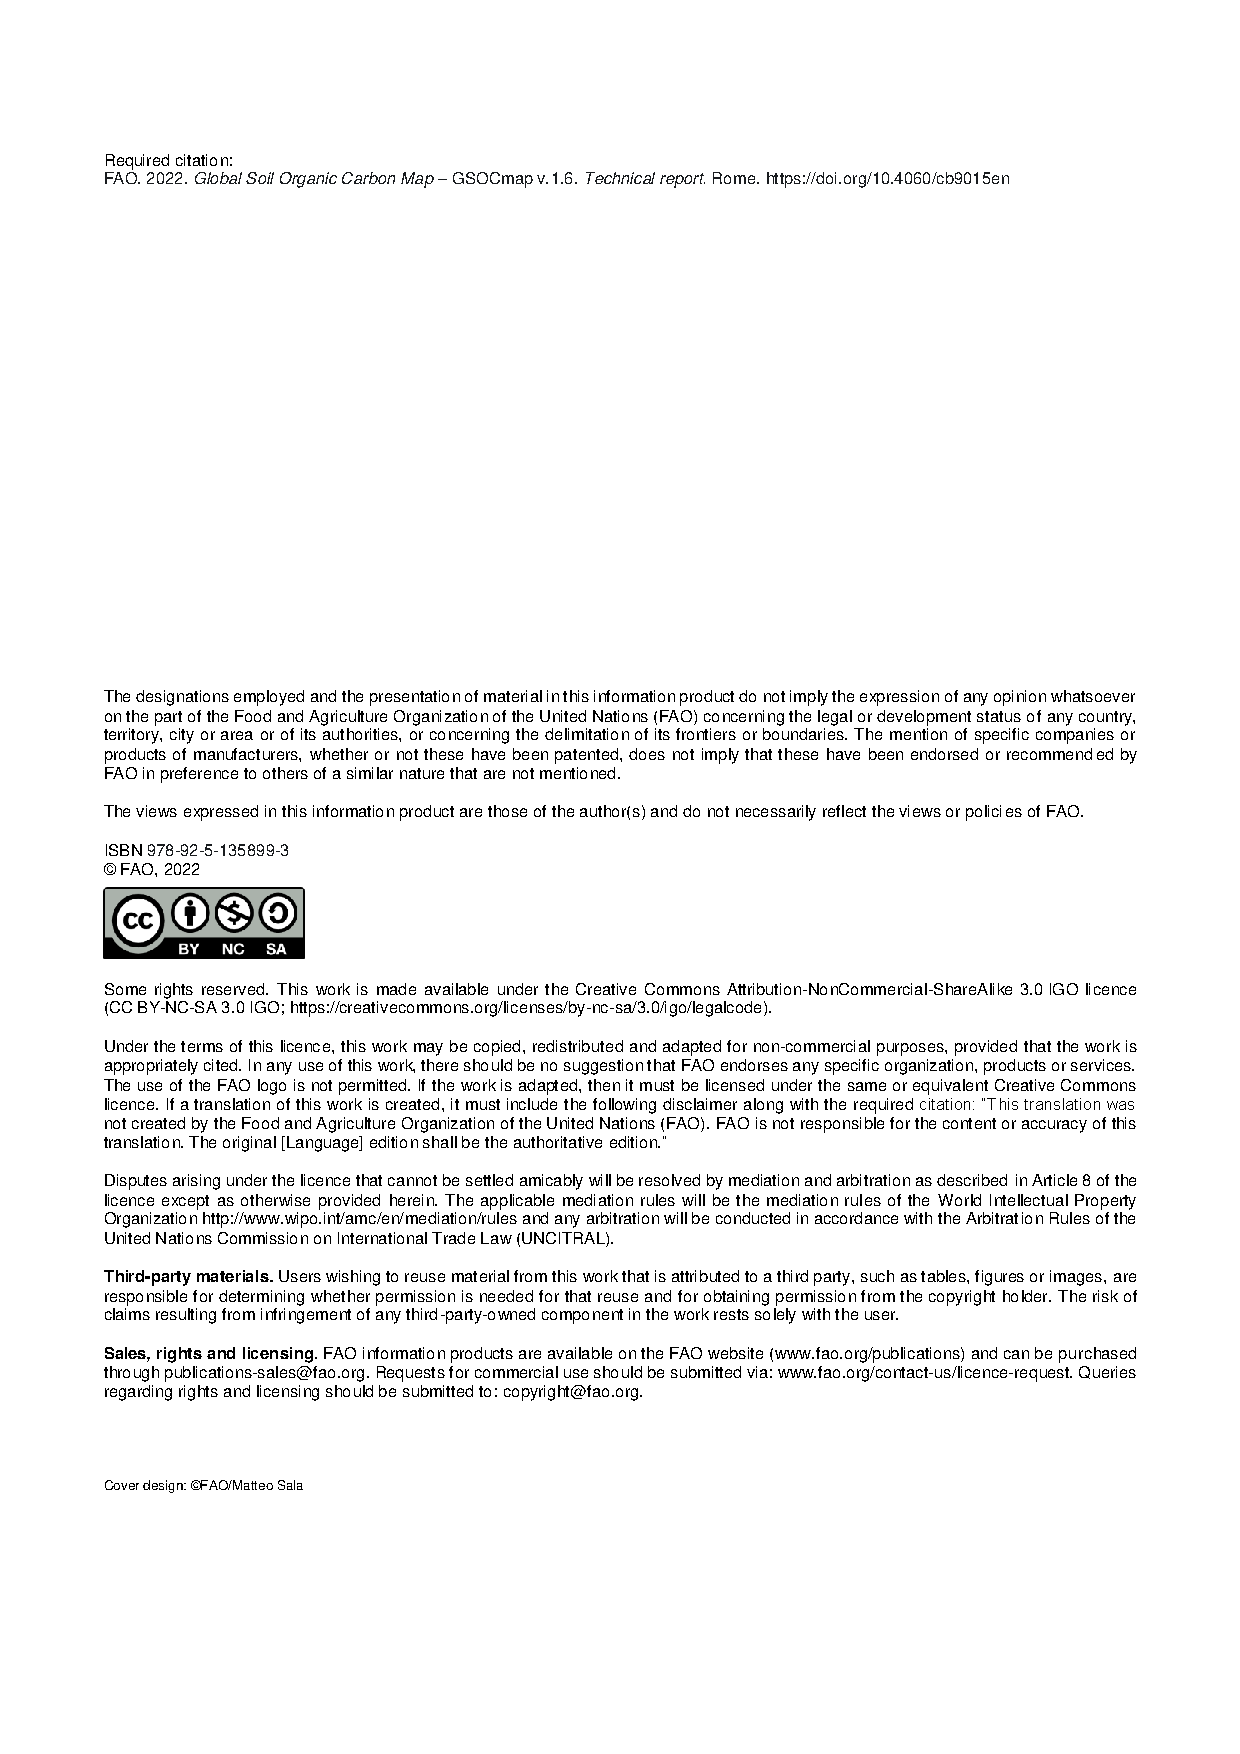
\includepdf{images/CB9015EN_Copyright Disclaimer_v2.pdf}


\hypertarget{licence}{%
\chapter*{Licence}\label{licence}}
\addcontentsline{toc}{chapter}{Licence}

Placeholder

\hypertarget{presentation}{%
\chapter{Presentation}\label{presentation}}

Placeholder

\hypertarget{global-soil-partnership}{%
\section{Global Soil Partnership}\label{global-soil-partnership}}

\hypertarget{country-driven-approach-and-tasks}{%
\section{Country-driven approach and tasks}\label{country-driven-approach-and-tasks}}

\hypertarget{how-to-use-this-book}{%
\section{How to use this book}\label{how-to-use-this-book}}

\hypertarget{training-material}{%
\section{Training material}\label{training-material}}

\hypertarget{soil-nutrients}{%
\chapter{Soil Nutrients}\label{soil-nutrients}}

Placeholder

\hypertarget{soil-properties-governing-nutrient-availability}{%
\section{Soil properties governing nutrient availability}\label{soil-properties-governing-nutrient-availability}}

\hypertarget{setting-up-the-software-environment}{%
\chapter{Setting-up the software environment}\label{setting-up-the-software-environment}}

Placeholder

\hypertarget{use-of-r-rstudio-and-r-packages}{%
\section{Use of R, RStudio and R Packages}\label{use-of-r-rstudio-and-r-packages}}

\hypertarget{obtaining-and-installing-r}{%
\subsection{Obtaining and installing R}\label{obtaining-and-installing-r}}

\hypertarget{obtaining-and-installing-rstudio}{%
\subsection{Obtaining and installing RStudio}\label{obtaining-and-installing-rstudio}}

\hypertarget{getting-started-with-r}{%
\subsection{Getting started with R}\label{getting-started-with-r}}

\hypertarget{r-packages}{%
\section{R packages}\label{r-packages}}

\hypertarget{gee---google-earth-engine}{%
\section{GEE - google earth engine}\label{gee---google-earth-engine}}

\hypertarget{digital-soil-mapping}{%
\chapter{Digital Soil Mapping}\label{digital-soil-mapping}}

Placeholder

\hypertarget{principles}{%
\section{Principles}\label{principles}}

\hypertarget{environmental-covariates}{%
\section{Environmental covariates}\label{environmental-covariates}}

\hypertarget{machine-learning-techniques}{%
\section{Machine learning techniques}\label{machine-learning-techniques}}

\hypertarget{mapping-of-soil-nutrients-and-associated-soil-attributes}{%
\section{Mapping of soil nutrients and associated soil attributes}\label{mapping-of-soil-nutrients-and-associated-soil-attributes}}

\hypertarget{arranging-soil-data-in-r}{%
\chapter{\texorpdfstring{Arranging soil data in \textbf{R}}{Arranging soil data in R}}\label{arranging-soil-data-in-r}}

Placeholder

\hypertarget{study-area-and-training-material}{%
\section{Study area and training material}\label{study-area-and-training-material}}

\hypertarget{georeferenced-topsoil-data}{%
\subsection{Georeferenced topsoil data}\label{georeferenced-topsoil-data}}

\hypertarget{soil-profile-data}{%
\subsection{Soil profile data}\label{soil-profile-data}}

\hypertarget{preproc}{%
\section{Format requirements of soil data}\label{preproc}}

\hypertarget{pre-processing-steps}{%
\section{Pre-processing steps}\label{pre-processing-steps}}

\hypertarget{set-the-scene-set-working-directory-packages-load-data}{%
\subsection{Set the scene (set working directory, packages, load data)}\label{set-the-scene-set-working-directory-packages-load-data}}

\hypertarget{basic-data-handling-operations}{%
\subsection{Basic data handling operations}\label{basic-data-handling-operations}}

\hypertarget{step-1-soil-data-preparation}{%
\chapter{Step 1: soil data preparation}\label{step-1-soil-data-preparation}}

Placeholder

\hypertarget{load-national-data}{%
\section{Load national data}\label{load-national-data}}

\hypertarget{data-quality-check}{%
\section{Data quality check}\label{data-quality-check}}

\hypertarget{calculation-of-pedo-transfer-functions}{%
\section{Calculation of pedo-transfer functions}\label{calculation-of-pedo-transfer-functions}}

\hypertarget{check-for-outliers}{%
\section{Check for outliers}\label{check-for-outliers}}

\hypertarget{harmonise-soil-layer-depths}{%
\section{Harmonise soil layer depths}\label{harmonise-soil-layer-depths}}

\hypertarget{harmonise-units}{%
\section{Harmonise units}\label{harmonise-units}}

\hypertarget{save-the-results}{%
\section{Save the results}\label{save-the-results}}

\hypertarget{step-2-download-environmental-covariates}{%
\chapter{Step 2: download environmental covariates}\label{step-2-download-environmental-covariates}}

Placeholder

\hypertarget{environmental-covariates-1}{%
\section{Environmental covariates}\label{environmental-covariates-1}}

\hypertarget{download-covariatesand-cropland-mask-with-google-earth-engine-gee}{%
\section{Download covariatesand cropland mask with Google Earth Engine (GEE)}\label{download-covariatesand-cropland-mask-with-google-earth-engine-gee}}

\hypertarget{assets}{%
\subsection{Assets}\label{assets}}

\hypertarget{define-the-region-of-interest-roi}{%
\subsection{Define the region of interest (ROI)}\label{define-the-region-of-interest-roi}}

\hypertarget{load-and-clip-the-covariates}{%
\subsection{Load and clip the covariates}\label{load-and-clip-the-covariates}}

\hypertarget{clean-holes-in-fpar-layers}{%
\subsection{Clean holes in FPAR layers}\label{clean-holes-in-fpar-layers}}

\hypertarget{visualize-and-export-the-covariates}{%
\subsection{Visualize and export the covariates}\label{visualize-and-export-the-covariates}}

\hypertarget{load-and-clip-the-copernicus-land-cover-map-and}{%
\subsection{Load and clip the Copernicus land cover map and}\label{load-and-clip-the-copernicus-land-cover-map-and}}

\hypertarget{reclassify-the-land-cover-map}{%
\subsection{Reclassify the land cover map}\label{reclassify-the-land-cover-map}}

\hypertarget{visualization-and-exporting-mask}{%
\subsection{Visualization and exporting mask}\label{visualization-and-exporting-mask}}

\hypertarget{run-and-export-in-gee}{%
\section{Run and export in GEE}\label{run-and-export-in-gee}}

\hypertarget{step-3-mapping-continuous-soil-properties}{%
\chapter{Step 3: Mapping continuous soil properties}\label{step-3-mapping-continuous-soil-properties}}

Placeholder

\hypertarget{mapping-soil-properties-with-random-forest}{%
\section{Mapping Soil Properties with Random Forest}\label{mapping-soil-properties-with-random-forest}}

\hypertarget{getting-prepared-to-map}{%
\section{Getting prepared to map}\label{getting-prepared-to-map}}

\hypertarget{covariate-selection}{%
\section{Covariate selection}\label{covariate-selection}}

\hypertarget{model-calibration}{%
\section{Model calibration}\label{model-calibration}}

\hypertarget{uncertainty-assessment}{%
\section{Uncertainty assessment}\label{uncertainty-assessment}}

\hypertarget{predicting-soil-attributes}{%
\section{Predicting soil attributes}\label{predicting-soil-attributes}}

\hypertarget{reporting-results}{%
\chapter{Reporting results}\label{reporting-results}}

Placeholder

\hypertarget{data-submission-form}{%
\section{Data submission form}\label{data-submission-form}}

\hypertarget{way-forward}{%
\chapter{Way forward}\label{way-forward}}

This technical manual provided step-by-step guidance on how to generate nutrient maps by means of quantile regression forest models within a digital soil mapping framework. The array of maps produced belongs to the first implementation phase of the GSNmap initiative and provides urgently needed data on nutrient stocks and soil properties that govern nutrient availability. Policymakers will be able to use this data to derive conclusions on where to concentrate efforts to improve soil and land management to strengthen agrifood systems.
The second phase of the GSNmap will make use of the first phase data products to derive nutrient budget maps. Therefore, additional datasets will be used for calculating input and output terms of nutrient stocks. The methodology is currently under development by the GSNmap working group. The technical documentation towards implementing the second phase will be made available in mid 2023.

\hypertarget{frequent-asked-questions-and-troubleshooting-answers}{%
\section{Frequent asked questions and Troubleshooting answers}\label{frequent-asked-questions-and-troubleshooting-answers}}

To be developed soon\ldots{}

\hypertarget{issues-in-the-gsnmap-technical-manual}{%
\section{Issues in the GSNmap Technical Manual}\label{issues-in-the-gsnmap-technical-manual}}

Please, report any issue in the GSNmap Technical Manual in its issues GitHub page \url{https://github.com/FAO-GSP/GSNmap-TM/issues}.

\hypertarget{get-help}{%
\section{Get help}\label{get-help}}

\begin{itemize}
\tightlist
\item
  Check the issues GitHub page \url{https://github.com/FAO-GSP/GSNmap-TM/issues}
\item
  Issues with R packages: search for solutions in \url{https://stackoverflow.com/}
\item
  \texttt{caret} package \url{https://topepo.github.io/caret/}
\item
  \texttt{terra} package \url{https://rspatial.org/terra/pkg/1-introduction.html}
\item
  \texttt{tidyverse} package \url{https://r4ds.had.co.nz/}
\item
  \texttt{sf} package \url{https://r-spatial.github.io/sf/}
\end{itemize}

If these links do not help you, contact us including the following text:

\emph{I am {[}FULL NAME{]}, responsible for producing the GSNmap of {[}COUNTRY{]}.}

\href{mailto:marcos.angelini@fao.org}{\nolinkurl{marcos.angelini@fao.org}}

\hypertarget{annex-i-compendium-of-r-scripts}{%
\chapter*{Annex I: Compendium of R scripts}\label{annex-i-compendium-of-r-scripts}}
\addcontentsline{toc}{chapter}{Annex I: Compendium of R scripts}

Placeholder

\hypertarget{script-0-introduction-to-r}{%
\section*{Script 0: Introduction to R}\label{script-0-introduction-to-r}}
\addcontentsline{toc}{section}{Script 0: Introduction to R}

\hypertarget{script-2-data-preparation}{%
\section*{Script 2: Data preparation}\label{script-2-data-preparation}}
\addcontentsline{toc}{section}{Script 2: Data preparation}

\hypertarget{scripts-3-download-environmental-covariates}{%
\section*{Scripts 3: Download environmental covariates}\label{scripts-3-download-environmental-covariates}}
\addcontentsline{toc}{section}{Scripts 3: Download environmental covariates}

\hypertarget{script-4-modelling-validation-and-prediction-using-soil-data-with-coordinates}{%
\section*{Script 4: Modelling, validation and prediction using soil data with coordinates}\label{script-4-modelling-validation-and-prediction-using-soil-data-with-coordinates}}
\addcontentsline{toc}{section}{Script 4: Modelling, validation and prediction using soil data with coordinates}

\hypertarget{annex-iii-mapping-without-point-coordinates}{%
\chapter*{Annex III: Mapping without point coordinates}\label{annex-iii-mapping-without-point-coordinates}}
\addcontentsline{toc}{chapter}{Annex III: Mapping without point coordinates}

Placeholder

\hypertarget{annex-iv-quality-assurance-and-quality-control}{%
\chapter*{Annex IV: Quality assurance and quality control}\label{annex-iv-quality-assurance-and-quality-control}}
\addcontentsline{toc}{chapter}{Annex IV: Quality assurance and quality control}

Placeholder

\hypertarget{step-1-completeness-of-layers}{%
\section*{Step 1: Completeness of layers}\label{step-1-completeness-of-layers}}
\addcontentsline{toc}{section}{Step 1: Completeness of layers}

\hypertarget{step-2-check-the-projection-and-resolution-of-all-data-products}{%
\section*{Step 2: Check the projection and resolution of all data products}\label{step-2-check-the-projection-and-resolution-of-all-data-products}}
\addcontentsline{toc}{section}{Step 2: Check the projection and resolution of all data products}

\hypertarget{step-3-check-the-extent}{%
\section*{Step 3: Check the extent}\label{step-3-check-the-extent}}
\addcontentsline{toc}{section}{Step 3: Check the extent}

\hypertarget{step-4-check-the-units-ranges-and-outliers}{%
\section*{Step 4: Check the units, ranges, and outliers}\label{step-4-check-the-units-ranges-and-outliers}}
\addcontentsline{toc}{section}{Step 4: Check the units, ranges, and outliers}

\hypertarget{qaqc-script}{%
\section*{QA/QC Script}\label{qaqc-script}}
\addcontentsline{toc}{section}{QA/QC Script}

\hypertarget{references}{%
\chapter*{References}\label{references}}
\addcontentsline{toc}{chapter}{References}

%\printindex
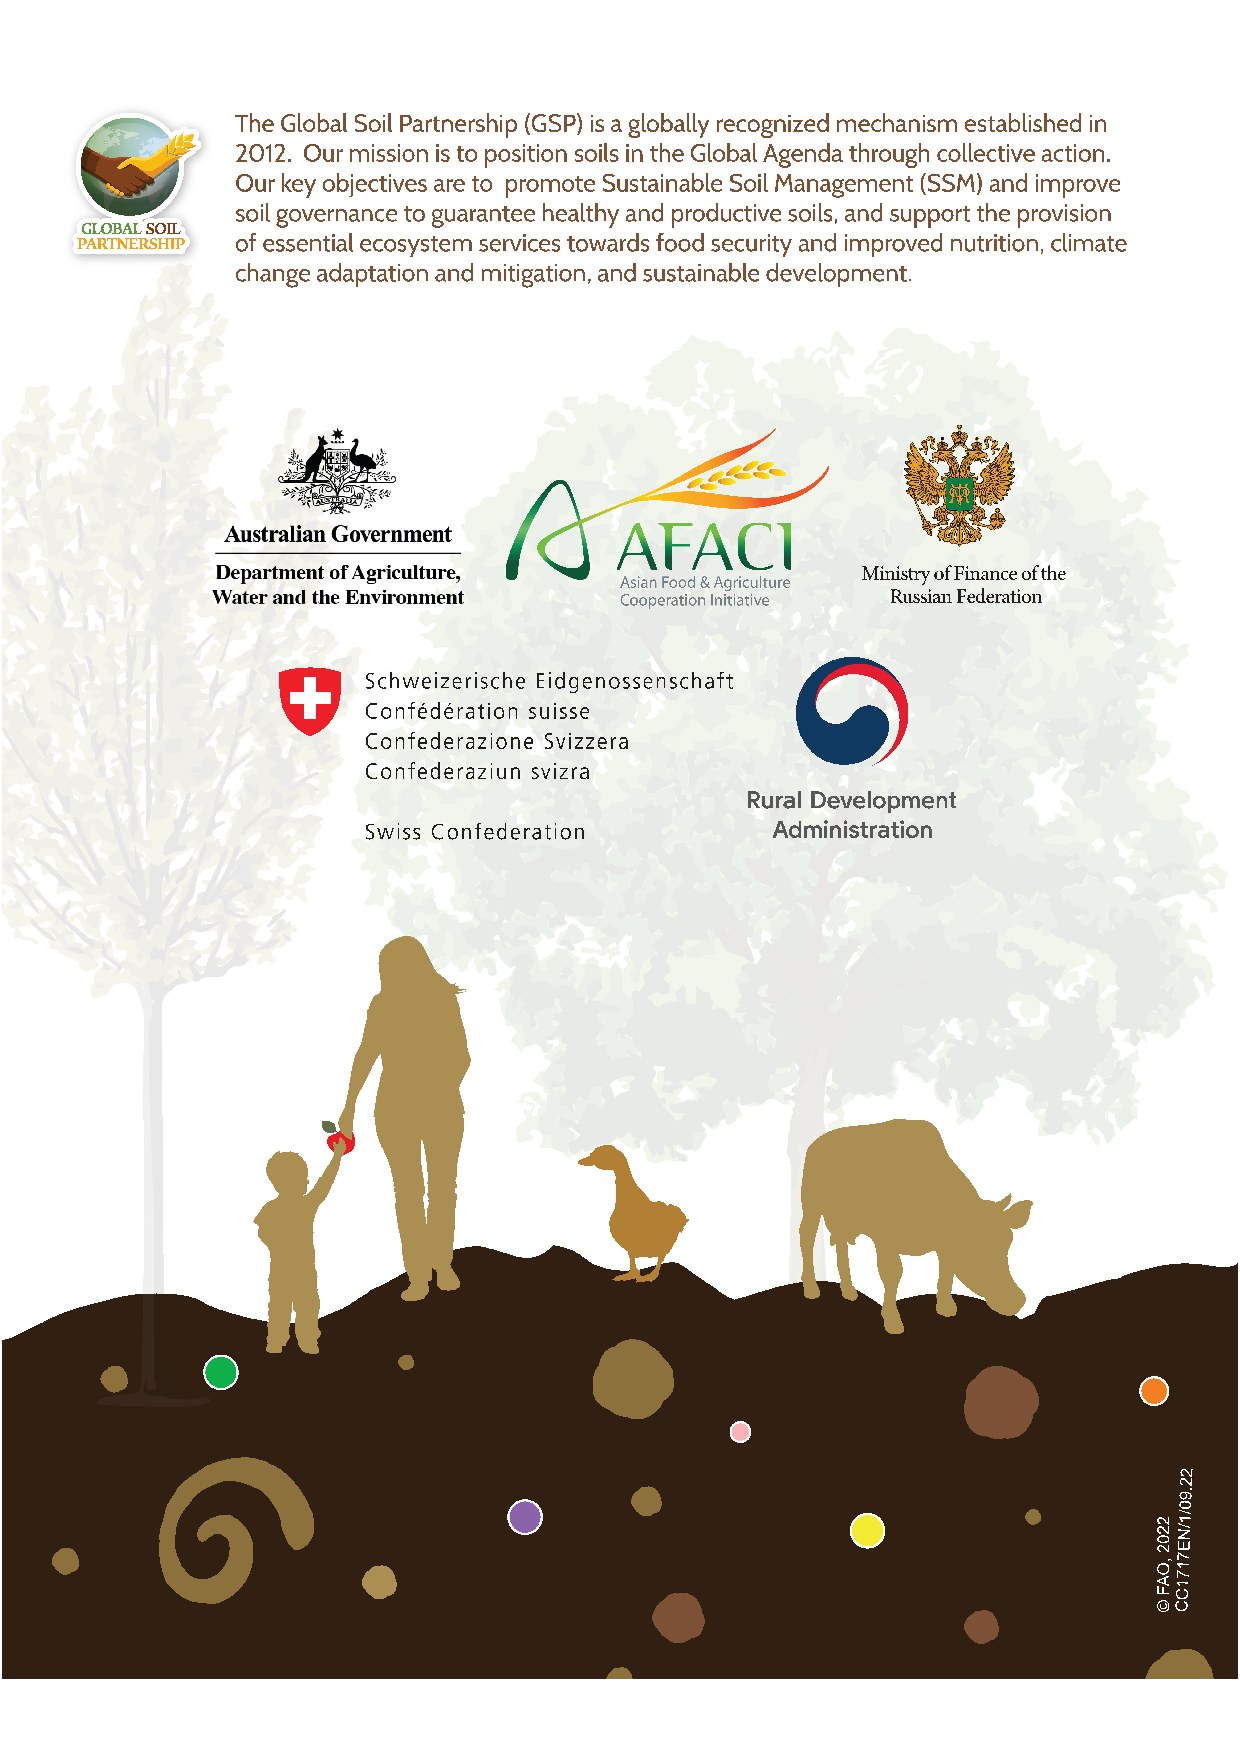
\includepdf{images/backcover.pdf}

\end{document}
